\documentclass[conference,a4paper]{IEEEtran}
\usepackage{amsmath,amssymb}
\usepackage{booktabs}
\usepackage{cite}
\usepackage[T1]{fontenc}
\usepackage{microtype}

\ifCLASSINFOpdf
  \usepackage[pdftex]{graphicx}
\else
  \usepackage[dvips]{graphicx}
\fi

% No automatic word breaks at line ends; extra stretch keeps the columns free of overfull lines.
\hyphenpenalty=10000
\exhyphenpenalty=10000
\tolerance=2000
\emergencystretch=1.5em

\begin{document}

\title{Inverse, Constrained and Physically Consistent Learning for the Design of a Low-Profile Wideband Patch Antenna}

\author{\IEEEauthorblockN{Pavan Mohan Neelamraju, Aakash Bansal, Will Whittow}
\IEEEauthorblockA{Wolfson School of Mechanical, Electrical and Manufacturing Engineering,\\
Loughborough University, Loughborough, United Kingdom, npavanmohan3@gmail.com}}

\maketitle

\begin{abstract}
In this paper, a low-profile, low-cost patch antenna for secure communication in the C-band is presented, together with a machine learning framework that returns its dimensions for a requested operating frequency. Two printed circuit boards, assembled without plated through holes in a 3-D printed fixture, are separated by an air gap that increases both the bandwidth and the efficiency, while the top board also acts as a protective radome. Four tightly coupled parasitic patches on the top board are excited by a driven patch, which is fed by a folded high-impedance microstrip line transformer. An impedance bandwidth of 4.4 to 5.4 GHz (20.4 percent), a gain of 8 to 10 dBi with a stable boresight pattern and a simulated radiation efficiency of 93 percent are obtained for an overall size of 0.98 by 0.98 by 0.085 free-space wavelengths at 4.9 GHz. To retarget its nine interdependent dimensions, 500 full-wave responses are converted into passive and causal equivalent circuits, a neural network ensemble predicts these circuits from the dimensions, and a constrained conditional generator inverts the ensemble. On unseen geometries, the surrogate halves the resonance frequency error of kriging and tree-based models without any passivity violation, and the inverse model returns diverse designs for any frequency between 4 and 7 GHz within seconds.
\end{abstract}

\vskip0.5\baselineskip

\begin{IEEEkeywords}
patch antenna, wideband, low profile, parasitic patches, inverse design, machine learning, equivalent circuit.
\end{IEEEkeywords}

\section{Introduction}
Microstrip patch antennas and arrays are widely used in mobile communication, radar systems, secure communication links and emergency services. They offer a low-profile planar geometry, a unidirectional radiation pattern, a variety of feeding techniques and easy integration with conformal and metallic platforms, since the inherent ground plane isolates the radiator from the mounting surface \cite{Garg2001, Balanis2016}. They are also cost-effective, because mature printed circuit board (PCB) fabrication replaces the machining of metals and plastics, and 3-D printed fixtures allow rapid progression from design to prototype. However, owing to the high quality factor of their thin cavity, patch antennas are inherently narrowband \cite{Lo2025}, and it remains challenging to increase their bandwidth without degrading the radiation pattern or raising the cost.

Several techniques enhance the bandwidth of patch antennas while preserving the radiation pattern and a low profile. Slot loading of the radiating patch, such as a U-shaped slot \cite{Wang2008}, introduces an additional resonance close to the fundamental mode in a single-layer structure, although the bandwidth is limited to 18\% and a relatively thick substrate of $0.07\lambda_0$ is required, which increases the weight and cost. Multimode patches, in which higher-order modes are excited alongside the fundamental mode, achieve 22--25\% with a profile below $0.05\lambda_0$ \cite{Lu2018, Jouybari2026}. However, mode mixing tilts the beam and raises the cross-polarisation in \cite{Lu2018}, while \cite{Jouybari2026} operates at millimetre-wave frequencies and would need a thicker substrate below 6~GHz. Stacked parasitic patches, electromagnetically coupled to a driven patch, increase both bandwidth and gain at the expense of an additional substrate layer \cite{Legay1993}. Dielectric loading, in which a high-permittivity ceramic feeder excites the patch, merges the slot, dielectric and patch resonances to achieve 45\%, but raises the profile to $0.11\lambda_0$, and its aperture-coupled feed makes the antenna sensitive to the mounting surface behind the ground plane \cite{Lo2025}.

Metasurface loading, in which a truncated array of unit cells is excited by a patch or a feeding aperture, provides 25--56\% with profiles below $0.09\lambda_0$ \cite{Lin2018, Lin2021, Zhou2022, Gao2026, Naik2025}. However, the metasurface is usually fed through a slot in the ground plane, which requires a feed line on the back face and typically three metal layers, and makes the antenna sensitive to the mounting surface \cite{Lin2021, Zhou2022, Gao2026}. Similarly, metasurface-loaded magneto-electric dipoles reach 42.8\% at $0.063\lambda_0$, but rely on via rows and multiple substrates \cite{Li2026}. The widest bandwidths are therefore obtained by combining several coupled resonances, at the cost of additional layers, vias or feed complexity, and with many interdependent dimensions that must be tuned simultaneously.

Machine learning (ML) now accelerates such multiparameter design \cite{akinsolu2024review}. Forward surrogates replace the full-wave solver inside an optimiser \cite{liu2014sadea, koziel2021inverse}, whereas inverse models map a target response directly to the dimensions through tandem networks \cite{liu2018tandem, gupta2023tandem} or conditional generative models \cite{labash2025generative, rather2026pixelated}. Three issues limit these models for resonant antennas. Coarse frequency sweeps alias high-$Q$ resonances, black-box regressors can predict non-passive responses with $|S_{11}|>1$, and the one-to-many inverse mapping lets unconstrained networks exploit surrogate errors \cite{ren2022benchmark}.

In this paper, a three-layer air-gap patch antenna with four tightly coupled parasitic patches is presented and combined with an inverse, constrained and physically consistent (ICP) learning framework that retargets its nine dimensions. The contributions are (i)~a low-profile wideband antenna without plated through holes that achieves 20.4\% bandwidth at $0.085\lambda_0$, (ii)~a passive-by-construction equivalent circuit representation and surrogate of its full-wave responses, and (iii)~a constrained inverse generator that returns fabrication-ready dimensions for any frequency between 4 and 7~GHz within seconds.

\section{Antenna Design}
\subsection{Antenna Configuration}
Fig.~\ref{Ant} shows the antenna. Two 60~mm $\times$ 60~mm PCBs with a substrate thickness of 0.79~mm are separated by an air gap $G$, which is set by a 3-D printed polylactic acid (PLA) fixture. The bottom PCB carries a driven patch of width $W$ and length $L$ above a solid ground plane. The patch is fed from a 50~$\Omega$ microstrip line through a folded high-impedance transformer of width $W_T$, meander width $C$ and length $L_T$, which matches the patch to the edge-mounted SMA connector without any plated through hole. The top PCB carries four identical parasitic patches of width $W_1$ and length $L_1$, separated by the gaps $S_x$ and $S_y$, and its substrate also serves as a protective radome.

\begin{figure}[!t]
\centering
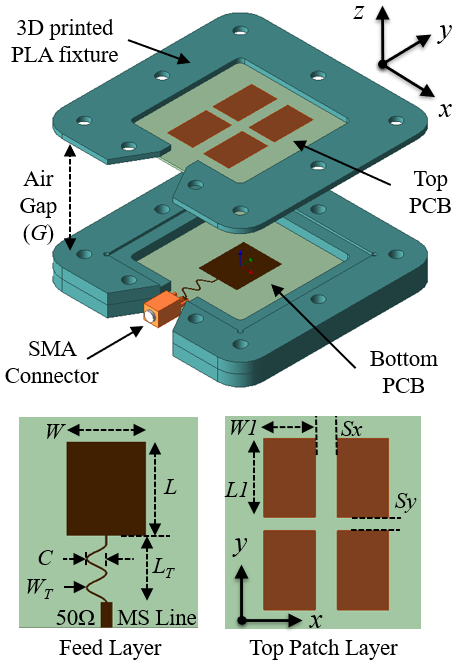
\includegraphics[width=0.56\columnwidth]{Pics/Ant.png}
\caption{Proposed antenna: exploded view of the assembly in its 3-D printed fixture, and dimensions of the feed layer and the top patch layer.}
\label{Ant}
\end{figure}

\subsection{Operating Principle and Performance}
The driven patch couples electromagnetically to the four parasitic patches across the air gap. The small gaps $S_x$ and $S_y$ couple the parasitic patches tightly, so that additional resonances appear close to the fundamental mode of the driven patch and merge into a single wide impedance band. The air gap lowers the effective permittivity and the quality factor of the stacked cavity, which increases both the bandwidth and the radiation efficiency \cite{Legay1993}, and the flat ground plane allows flush mounting on a platform. The antenna provides an impedance bandwidth of 4.4--5.4~GHz (20.4\%), a stable boresight radiation pattern with a gain of 8--10~dBi, E-plane and H-plane beamwidths of 58\textdegree--46\textdegree{} and 70\textdegree--62\textdegree{}, and a simulated radiation efficiency of 93\%. The overall size is 60~mm $\times$ 60~mm $\times$ 5.2~mm, that is $0.98\lambda_0 \times 0.98\lambda_0 \times 0.085\lambda_0$ at 4.9~GHz, excluding the fixture.

\subsection{Design Variables}
Table~\ref{tab:vars} lists the nine independent dimensions and their ranges. The length of the parasitic patches is parametrised as $L_1 = W_1 + E$ with $E \ge 0.5$~mm, the meander position follows $L$, and the substrate thickness and board size are fixed. A sensitivity analysis of the trained surrogate of Section~\ref{sec:icp} shows that $C$ and $L$ dominate the resonance frequency, which they change by about 0.29 and 0.20~GHz per millimetre, respectively. Because all nine dimensions interact, tuning one at a time is slow, which motivates the learning framework.

\begin{table}[!t]
\centering
\caption{Design Variables and Sampled Ranges}
\label{tab:vars}
\footnotesize
\setlength{\tabcolsep}{4pt}
\begin{tabular}{llc}
\toprule
Symbol & Description & Range (mm) \\
\midrule
$G$ & air gap between the PCBs & 1.5--5.0 \\
$W$, $L$ & width and length of the driven patch & 10--23, 15--23 \\
$W_T$ & width of the folded transformer & 0.2--1.5 \\
$C$ & meander width of the transformer & 0.5--4.0 \\
$W_1$ & width of the parasitic patches & 8--17 \\
$L_1-W_1$ & elongation $E$ of the parasitic patches & 0.5--8.0 \\
$S_x$, $S_y$ & gaps between the parasitic patches & 0.2--5.0 \\
\bottomrule
\end{tabular}
\end{table}

\section{ICP Learning Framework}
\label{sec:icp}
Fig.~\ref{fig:framework} summarises the framework. Five hundred designs were sampled uniformly over the ranges of Table~\ref{tab:vars} and simulated in Ansys HFSS from 4 to 7~GHz at 31 frequency points, taking 161~s each on average (22.3~h in total). All results below use one fixed five-fold split by geometry, so every error refers to unseen designs.

\begin{figure*}[!t]
\centering
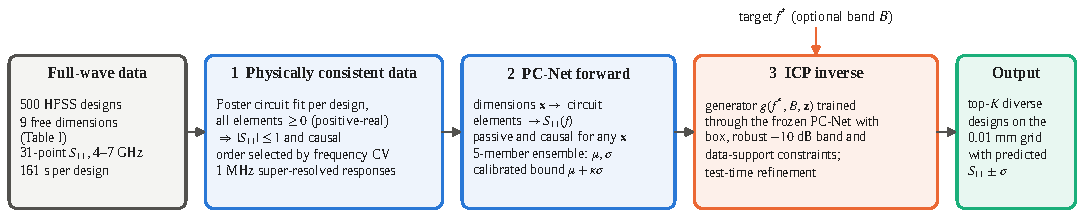
\includegraphics[width=\textwidth]{figures/fig_framework.pdf}
\caption{ICP framework: physically consistent data representation, passive-by-construction forward ensemble (PC-Net) and constrained inverse generator with test-time refinement.}
\label{fig:framework}
\end{figure*}

\subsection{Physically Consistent Representation}
Each simulated response is fitted with
\begin{align}
S_{11}(f)&=e^{-j2\pi f\tau}\,\frac{Z(f)-1}{Z(f)+1},\label{eq:foster}\\
Z(f)&=R_0+jaf-\frac{jb}{f}+\sum_{k=1}^{K}\frac{R_k}{1+jQ_k\left(\frac{f}{f_k}-\frac{f_k}{f}\right)},\nonumber
\end{align}
where $Z$ is normalised to 50~$\Omega$ and all elements are non-negative. The impedance is then positive-real, so $|S_{11}|\le 1$ and causality hold for every parameter value. A multistart bounded least-squares fit is computed for $K=2,\dots,5$ resonators. The order $K$ is selected for each design by fitting the even-indexed samples and scoring the odd-indexed ones, and the selected model is refitted to all 31 samples and evaluated on a 1~MHz grid. This yields the resonance frequency $f_r$, the minimum $|S_{11}|$ and the $-10$~dB band of every design.

\subsection{PC-Net Forward Ensemble}
A three-layer perceptron with 128 units per layer maps the nine scaled dimensions to the elements of (\ref{eq:foster}) with six resonators through softplus and sigmoid heads, followed by the differentiable decoder. Passivity and causality therefore hold by construction rather than through a penalty \cite{torun2020causal}, and the decoder exposes interpretable resonance frequencies and quality factors. The network is trained on the simulated samples and on the 10~MHz responses of Section~\ref{sec:icp}-A with a complex-error plus dB-error loss. Five members with different validation splits form a deep ensemble \cite{lakshminarayanan2017ensembles} with mean $\mu(f)$ and spread $\sigma(f)$ of $|S_{11}|$ in dB, calibrated on out-of-fold data so that $\mu+\kappa\sigma$ with $\kappa=1.22$ is an empirical one-sided 84\% bound.

\subsection{Constrained Inverse Generator}
A conditional generator $\mathbf{u}=g(f^*,B,\mathbf{z})$, with latent vector $\mathbf{z}\sim\mathcal{N}(\mathbf{0},\mathbf{I}_4)$ and a sigmoid output that keeps every dimension inside its range, is trained through the frozen ensemble (tandem learning \cite{liu2018tandem}) to minimise
\begin{align}
\mathcal{L}=&\big\langle[\mu+\kappa\sigma+11]_+^2\big\rangle_{B}+\lambda_s\big[d_{\rm kNN}(\mathbf{u})-d_{\max}\big]_+^2\nonumber\\
&-\lambda_d\,\|\mathbf{u}_1-\mathbf{u}_2\|/\|\mathbf{z}_1-\mathbf{z}_2\|,
\end{align}
where $\langle\cdot\rangle_B$ averages over the requested band $[f^*-B/2,\,f^*+B/2]$. The first term enforces $|S_{11}|\le-10$~dB with a 1~dB margin on the calibrated bound. The second term keeps the designs inside the sampled domain, with $d_{\max}$ the 95th percentile of the nearest-neighbour distance between simulated designs. The third term rewards distinct designs for distinct latent vectors, which preserves multiple solutions of the one-to-many problem. At test time, 128 candidates, half from $g$ and half uniform, are refined for 100 Adam steps on the same objective, snapped to the 0.01~mm grid and re-evaluated on a 5~MHz grid. They are ranked by calibrated feasibility, then by whether the calibrated band centred on $f^*$ is at least $\max(0.2~\mathrm{GHz},B)$ wide, about twice the resonance frequency error of the surrogate, and then by the calibrated margin, and a diversity filter returns the top five designs. A NumPy implementation of the search takes about 6~s on a two-core CPU.

\section{Results}
\subsection{Super-Resolution of Coarse Sweeps}
Fitting the 16 even-indexed samples of every design and predicting the 15 held-out samples, the equivalent circuit gives a mean absolute error (MAE) of 0.11~dB, against 0.35--1.24~dB for linear, spline and piecewise cubic interpolants. Near resonance ($|S_{11}|\le-6$~dB), its error of 0.31~dB is 7.2 times lower than that of the best interpolant. It makes 20 wrong $-10$~dB decisions over the 500 designs, against at least 165 for the interpolants, and never violates passivity, whereas both cubic splines do. Fig.~\ref{fig:sr} shows the design with the deepest sampled resonance. At the held-out 5.9~GHz sample, the full-wave result is $-35.1$~dB, linear interpolation gives $-11.5$~dB and the equivalent circuit predicts $-33.0$~dB. Over the data set, 293 designs meet $-10$~dB on the 1~MHz grid against 265 on the raw grid, and 91 designs have a true minimum more than 3~dB below their best sample.

\begin{figure}[!t]
\centering
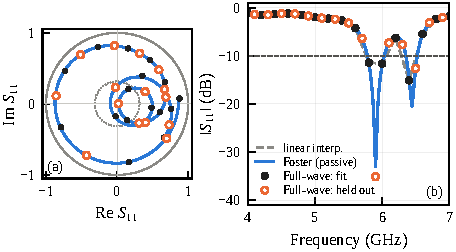
\includegraphics[width=\columnwidth]{figures/fig_extraction.pdf}
\caption{Frequency hold-out test on the design with the deepest sampled resonance: (a) Smith chart and (b) magnitude. The equivalent circuit is fitted to the filled samples only.}
\label{fig:sr}
\end{figure}

\subsection{Forward Accuracy on Unseen Geometries}
\label{sec:fwd}
Table~\ref{tab:fwd} compares PC-Net with Extra Trees, kriging and multilayer perceptron (MLP) ensembles trained on the same folds. PC-Net lowers the MAE from 1.25 to 0.84~dB, the error near resonance from 4.13 to 2.61~dB and the resonance frequency error from 231 to 118~MHz, with 62\% of the resonances predicted within 50~MHz. The dB-domain models detect almost none of the $-10$~dB samples (F1 score $\le 0.10$), whereas PC-Net reaches an F1 score of 0.62. In a screening test, every model ranks the 100 unseen geometries of each test fold at every frequency, and the five top-ranked designs are checked against their simulated response. The picks of PC-Net meet $-10$~dB in 55\% of cases, against 27\% for the best baseline and a 4.7\% base rate, and the calibrated rule $\mu+\kappa\sigma\le-10$~dB is correct in 87.5\% of its decisions. The MLP on real and imaginary parts violates passivity in 9.3\% of its predictions, and PC-Net in none (Fig.~\ref{fig:fwd}).

\begin{table}[!t]
\centering
\caption{Forward Surrogates on Unseen Geometries (Five-Fold Cross-Validation)}
\label{tab:fwd}
\footnotesize
\setlength{\tabcolsep}{2.4pt}
\begin{tabular}{lccccc}
\toprule
Model & MAE (dB) & $f_r$ err. (MHz) & F1 & P@5 (\%) & $|S_{11}|{>}1$ (\%) \\
\midrule
Extra Trees & 1.48$\pm$0.08 & 231 & 0.02 & 19 & 0.0 \\
Kriging & 1.25$\pm$0.05 & 258 & 0.10 & 27 & 0.7 \\
MLP, dB & 1.52$\pm$0.09 & 264 & 0.06 & 25 & 3.7 \\
MLP, Re/Im & 2.59$\pm$0.25 & 495 & 0.28 & 21 & 9.3 \\
\textbf{PC-Net} & \textbf{0.84$\pm$0.12} & \textbf{118} & \textbf{0.62} & \textbf{55} & \textbf{0.0} \\
\bottomrule
\end{tabular}\\[2pt]
\parbox{\columnwidth}{\scriptsize MAE: mean$\pm$std over folds; P@5: fraction of the five top-ranked unseen designs that meet $-10$~dB at the queried frequency (base rate 4.7\%).}
\end{table}

\begin{figure*}[!t]
\centering
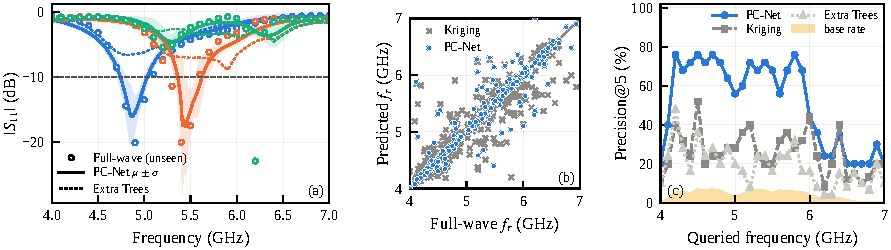
\includegraphics[width=\textwidth]{figures/fig_forward.pdf}
\caption{PC-Net on unseen geometries: (a) median-error designs from three bands, with PC-Net mean $\pm\sigma$ and Extra Trees; (b) resonance frequency parity against kriging; (c) screening precision versus queried frequency, with the base rate shaded.}
\label{fig:fwd}
\end{figure*}

\subsection{Inverse Design}
Table~\ref{tab:inv} uses 100 specifications $(f_c,B)$ achieved by unseen test-fold designs, which are therefore feasible, and 70 single-frequency targets from 4.2 to 6.8~GHz. The proposed dimensions are scored by a reference PC-Net ensemble trained on all 500 designs with different seeds, since kriging detects fewer than 7\% of the matched samples. The optimism, that is the reference minus the self-predicted $|S_{11}(f^*)|$, measures the exploitation of surrogate errors.

\begin{table}[!t]
\centering
\caption{Inverse Design on Held-Out Specifications}
\label{tab:inv}
\footnotesize
\setlength{\tabcolsep}{4pt}
\begin{tabular}{lcccc}
\toprule
Method & Spec. (\%) & Calib. (\%) & Opt. (dB) & Time (s) \\
\midrule
Catalogue retrieval & 80 & 49 & -- & $<$0.01 \\
Direct inverse MLP & 6 & 1 & 0.0 & $<$0.01 \\
Conditional VAE & 8 & 1 & 0.2 & $<$0.01 \\
Tandem (unconstrained) & 90 & 33 & 2.9 & $<$0.01 \\
Constr. opt., random init. & 98 & 55 & 3.3 & 1.77 \\
ICP generator only & 96 & 60 & 3.0 & 0.07 \\
ICP w/o constraints & 94 & 58 & 6.2 & 1.62 \\
\textbf{ICP (proposed)} & \textbf{98} & \textbf{65} & 3.8 & 1.76 \\
\bottomrule
\end{tabular}\\[2pt]
\parbox{\columnwidth}{\scriptsize Spec.: $|S_{11}|\le-10$~dB over the band of the 100 held-out specifications; Calib.: reference $\mu+\kappa\sigma\le-10$~dB over all 170 targets; Opt.: median optimism.}
\end{table}

\begin{table}[!t]
\centering
\caption{Top-Ranked ICP Designs (Dimensions in mm)}
\label{tab:designs}
\scriptsize
\setlength{\tabcolsep}{2.4pt}
\begin{tabular}{lccccccc}
\toprule
$f^*$ (GHz) & 4.5 & 4.9$^\dagger$ & 5.0 & 5.5 & 5.8 & 6.2 & 6.6 \\
\midrule
$G$ & 2.87 & 1.78 & 3.24 & 4.46 & 3.64 & 1.73 & 1.82 \\
$W$ & 17.89 & 11.93 & 14.95 & 17.27 & 12.15 & 14.83 & 13.02 \\
$L$ & 21.09 & 18.61 & 19.51 & 17.88 & 17.32 & 18.81 & 18.12 \\
$W_T$ & 1.22 & 1.36 & 1.05 & 1.18 & 0.78 & 1.04 & 1.08 \\
$C$ & 1.06 & 2.83 & 0.90 & 0.96 & 0.97 & 3.31 & 3.12 \\
$W_1$ & 15.47 & 15.35 & 13.47 & 11.20 & 10.88 & 13.39 & 13.17 \\
$L_1$ & 17.05 & 20.42 & 17.94 & 15.30 & 14.23 & 20.62 & 19.91 \\
$S_x$ & 1.09 & 0.34 & 0.96 & 2.02 & 1.34 & 0.47 & 0.38 \\
$S_y$ & 1.29 & 4.70 & 3.81 & 3.77 & 3.48 & 4.28 & 4.56 \\
\midrule
$|S_{11}(f^*)|$ & $-22{\pm}2$ & $-13{\pm}2$ & $-24{\pm}3$ & $-23{\pm}2$ & $-27{\pm}9$ & $-22{\pm}2$ & $-25{\pm}2$ \\
$f_L$ (GHz) & 4.32 & 4.35 & 4.70 & 5.27 & 5.54 & 6.05 & 6.46 \\
$f_H$ (GHz) & 4.75 & 5.51 & 5.54 & 5.92 & 6.10 & 6.37 & 6.76 \\
\bottomrule
\end{tabular}\\[2pt]
\parbox{\columnwidth}{\scriptsize $^\dagger$Requested band $B=1$~GHz (4.4--5.4~GHz); all other targets maximise the band centred on $f^*$. $|S_{11}(f^*)|$: mean$\pm\sigma$ in dB; $f_L$--$f_H$: predicted mean $-10$~dB band.}
\end{table}

The direct inverse MLP and the conditional variational autoencoder (VAE), both trained on the data alone, succeed in at most 10\% of the cases, because the mapping is one-to-many. The generator alone meets 96\% of the specifications in 0.07~s, but returns a single solution. The complete ICP search meets 98\% of the specifications, returns five diverse designs per query in 1.8~s and has the highest calibrated success, 65\%, against 55\% for constrained optimisation from random starts and 33\% for the unconstrained tandem network. Removing the robust and support constraints raises the median optimism from 3.8 to 6.2~dB. Retrieval from the simulated catalogue succeeds in 80\% of the specifications, but above 6.5~GHz at most seven designs meet $-10$~dB at the target. Fig.~\ref{fig:inv}(a) shows the benefit of the learned generator: initialised from it, the search reaches 74\% calibrated success without any refinement, against 46\% for random initialisation.

\begin{figure*}[!t]
\centering
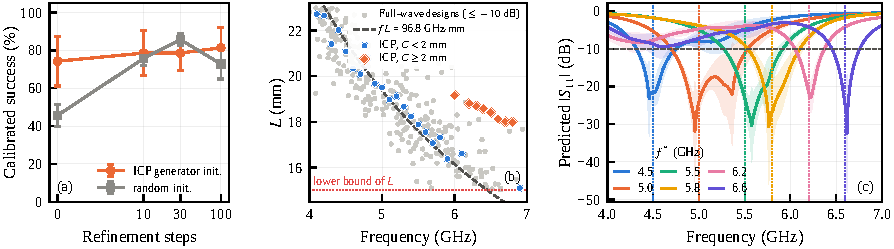
\includegraphics[width=\textwidth]{figures/fig_inverse.pdf}
\caption{Inverse design: (a) calibrated success of the top-ranked design on the 70 frequency targets versus refinement steps (mean $\pm$ standard error over five folds); (b) driven patch length of the top-ranked design for targets from 4.1 to 6.9~GHz, against the matched full-wave designs and the fitted law $fL=$~const.; (c) predicted $|S_{11}|$ of the six frequency-targeted designs of Table~\ref{tab:designs} (mean $\pm\sigma$).}
\label{fig:inv}
\end{figure*}

The designs are also physically consistent beyond passivity. In Fig.~\ref{fig:inv}(b), the designs with $C<2$~mm follow the half-wavelength scaling $fL=97.3\pm2.9$~GHz$\cdot$mm of the driven patch, close to $96.8\pm5.1$~GHz$\cdot$mm for the simulated designs, although this law was never imposed. Since the scaling would require $L$ below its 15~mm limit above 6.4~GHz, the method switches from 6~GHz upward to a second family with a large $C$ and a small $G$, which is also present in the data. Table~\ref{tab:designs} lists the top-ranked design for six targets and for the band of the reported antenna, 4.4--5.4~GHz. For this specification, the predicted mean band of 4.35--5.51~GHz covers the requirement, whereas the calibrated bound narrows it to 4.42--5.22~GHz, which places the specification at the edge of the learned domain.

\section{Conclusion}
A low-profile wideband patch antenna without plated through holes has been presented, in which four tightly coupled parasitic patches above an air gap provide 20.4\% bandwidth, 8--10~dBi gain and 93\% simulated efficiency at a profile of $0.085\lambda_0$. An inverse, constrained and physically consistent learning framework, built from 500 full-wave simulations, retargets its nine dimensions. Passivity and causality encoded in the data and the surrogate halve the resonance frequency error of conventional surrogates, and the constrained generator returns diverse, physically scaled designs for any frequency between 4 and 7~GHz within seconds.

\bibliographystyle{IEEEtran}
\bibliography{refs}

\end{document}
